%!TEX root = ../main.tex

\section{Introduction}
\label{s:intro}

Poor data quality is estimated to cost the US economy more than \$600 billion
per year~\cite{eckerson2002} and erroneous price data in retail databases
alone cost the US consumers \$2.5 billion each year~\cite{Fan2008}. 
\ewu{
It is possible to use tools to fix existing errors in the database.
However, databases are dynamic -- applications and users constantly generate and execute queries that modify the database.
Any errors in the queries can easily propagate in complex ways and spread errors throughout the database that are hard to reason about.
Fixing the errors that have been found in the current data is not enough because not all of the errors may have been found because the source of the error could be buried deep in the past.
No tools exist to both {\it find} the erroneous queries and provide {\it fixes/explanations}.
}
While data cleaning tools can purge datasets of many errors before the data is
used, applications and users interacting with the data can introduce new
errors. Mistakes in data entry and erroneous updates often affect datasets in
complex ways and result in data errors that are obscure and hard to trace and
correct. Traditional data cleaning approaches are not well-suited for this
purpose: While they provide general-purpose tools to identify and rectify
anomalies in the data, they are not designed to diagnose the causes of these
errors, which are rooted in erroneous updates.

Improving data quality and correcting data errors has been an important focus
for data management research. Yet, handling new errors, introduced during
regular database interactions, has received little attention. Integrity
constraints~\cite{Khoussainova2006} can guard against some improper updates,
but only if the data falls outside rigid, predefined ranges. Certificate-based
verification~\cite{Chen2011} is impractical as it requires users to answer
challenge questions before allowing the updates, and it is not applicable to
updates initiated by applications.


\ewu{
In this paper, we argue for a new type of data error diagnosis called Data Fracking 
that targets data modification queries deep in the database transaction log.
In contrast to existing data cleaning and explanation approaches that aim to
detect, fix, or explain errors in the current database, Data Fracking both identifies the
root causes of the errors as past query transactions that {\it introduced} the errors
into the database, and proposes modifications to those anomalous queries that
fix the current errors.  By introducing a {\it new dimension} to data error diagnosis,
data fracking can lead to the identification of additional discrepancies that would
have otherwise remained undetected.
}
In this paper, we present a specialized data cleaning framework, \sys, that
specifically targets errors in update workloads. In contrast to traditional
data cleaning techniques that aim to identify errors in the data directly, the
goal of \sys is to \emph{explain} how the errors occurred. Our goal is not
simply to provide explanations; identifying how an error was introduced to a
dataset, can lead to the identification of additional discrepancies that would
have otherwise remained undetected.

\begin{example}[Incorrect insurance premiums]
    After negotiations with health insurance companies, an employer achieved
    reductions in the premium rates for the upcoming year, for employees at
    levels 1-4. The administrator who updated the employee database mistakenly
    implemented the new policy for employees at levels 1-3, due to the
    incorrect predicate \texttt{level < 4}.
    
    In subsequent months, level 4 employees who noticed that their premiums
    had not been reduced as expected, notified HR of the error. HR corrected
    employees' records on a case-by-case basis, obscuring the real cause of
    the problem, and making it harder to identify and correct the error for
    other employees.
    
    To make matters worse, subsequent queries that calculated employee
    withholdings, resulted in misestimation of the company's revenue and
    incorrect allocation of bonuses. Correcting errors in the employee
    premiums is no longer sufficient, as these errors have already had a
    larger effect on the data.
    
        \alex{Needs to be more realistic and convincing.  Ideally grounded on a real scenario.  Do we have more specific info for the use-cases?}
\end{example}

\ewu{In reality, the problems presented to HR were simply a small sample
of the errors stemming from the anomalous query.  Once HR fixes the errors,
there are still a potentially large number of employees whose premiums are incorrect that have
simply not complained to HR yet.
it is thus desirable to, given HR's fixes, identify candidate queries that may have been the source
of the error, propose fixes, and subsequently identify the other employees whos premiums are in error.

This problem is fundamentally challenging because ??? and must solve several challenging subproblems.
1) rollback  2) fix generation  3) fix picking (if there are multiple possible fixes) 4) performance.
}



% these characterize the problem
\ewu{Would say these nicely characterize the problem, not necessarily challenges.}
Diagnosing data errors stemming from incorrect updates raises three major
challenges that make existing data cleaning techniques not applicable.



\begin{description}[leftmargin=*, topsep=0mm, itemsep=0mm]
    
    \item[Obscurity.] Detection of the resulting errors in the data often
    leads to partial fixes that further complicate the eventual diagnosis and
    resolution of the problem. For example, a transaction implementing a
    change in the state tax law updated tax rates using the wrong rate,
    affecting a large number of consumers. This causes a large number of
    complaints to a call center, but each customer agent usually fixes each
    problem individually, which ends up obscuring the source of the problem.
    
    \item[Large impact.] Erroneous queries cause errors in a large scale. The
    potential impact of the errors is high, as manifested in several
    real-world cases~\cite{Yates10, Grady13, sakalerrors}. Further, errors
    that remain undetected for a significant amount of time can instigate
    additional errors, even through valid updates. This increases both their
    impact, and their obscurity.
    
    \item[Systemic errors.] The errors created by bad queries are
    \emph{systemic}: they have common characteristics, as they share the same
    cause. The link between the resulting data errors is the query that
    created them; cleaning techniques should leverage this connection to
    diagnose and fix the problem. Diagnosing the cause of the errors, will
    achieve systematic fixes that will correct all relevant errors, even if
    they have not been explicitly identified.
    
\end{description}
% 
\sys addresses these challenges by analyzing the queries that operated on a
dataset in an efficient and scalable manner. More concretely, we make the
following contributions:


% The goal of this paper is to design effective query
% diagnosis techniques and identify possible fixes for query errors. We
% model the problem assuming a log of update workloads over a database,
% and a set of complaints that identify errors in the final database
% state. We organize our contributions as follows:

\ewu{really like this organization}.

\begin{itemize}[leftmargin=*, topsep=0mm, itemsep=0mm]      
    \item We formalize the Data Fracking problem of diagnosing a set of errors using log
    histories of updates that operated on the data. Given a set of 
    \emph{complaints} as representations of data discrepancies in the current
    state of a dataset, \sys identifies the queries in the log that require the  minimal
    amount of changes that would resolve all of the complaints (Section~\ref{???}).
      
    \item We provide an exact error-diagnosis solution through a non-trivial
    transformation of the problem to a mixed integer program (MIP) that
    analyzes the data provenance of the erroneous tuples at the attribute
    level. Our approach employs state-of-the-art MIP solvers to identify
    optimal diagnoses that are guaranteed to resolve all complaints, and is
    tolerant to incomplete information (missing complaints)
    (Section~\ref{???}).
    
    \item While modern solvers can handle large numbers of variables and
    constraints, eventually, they fail to scale to very large datasets and
    large query logs. We present several performance optimizations that allow
    our diagnostic methods to scale, in many cases without affecting the
    quality of the produced solutions (Section~\ref{???}).
    
    \item We extend our framework to also handle false positives: complaints
    that mistakenly identify data as erroneous. We define the notion of
    complaint \emph{density}, which is a query-driven measure of closeness of
    a complaint to other complaints. The main intuition of our approach is
    that complaints of low density are likely false positives and thus can be
    safely ignored (Section~\ref{???}).
    
    \item We experimentally evaluate the effectiveness and efficiency of our
    methods against real-world and synthetic datasets and query logs. We
    demonstrate that \xxx{... to be completed when we know what we have}
    (Section~\ref{???}).
\end{itemize}


\deprecate{
While exploring data, its natural to come across surprising or unexpected data.
For example, visual data analysis explores the current state of the database and users may be surprised by outliers in a visualization.
Similarly, enterprise customers (e.g., billing) may find outliers in their monthly bills and be surprised by the amount they are asked to pay.

When presented with these surprises, users want to better understand the reasons behind the anomalies.
A recent wave of research focuses on deriving predicate-based explanations for outliers for statistical aggregation queries.
For example, if the user wants to understand why the total sales in the past few months have gone up, these systems can general explanations such as ``most related to customers in California between the ages of 12 to 18.''
However, these approaches simply generate predicates that describe {\it current state} of the database, and do not resolve {\it how} the anomalous data came to be.

Specifically, the user may also be interested to understand which past database modification was responsible for these explanations.
Describe why this makes sense to want.  In this form of the problem, we are interested in historical database queries whose modifications, when propogated to the current database state, 
The goal is to provide diagnostic tools that can peer into past transactions.


In this paper, we approach anomaly explanation from the persepctive of the query log and seek to
both {\it identify}  historical database modification queries that most likely caused user complaints 
in the current state of the database, and suggest replacement queries that will resolve these complaints.
We call this problem the {\it Query-based Complaint-Satisfaction Problem}.

Given a database query log and a set of {\it complaints} (e.g., tuple 1's attribute B should be 20\% lower) about records in the current state of the database,
we seek to identify the subset of queries in the log that, by modifying their parameters and propogating the new effects of the queries, 
will best resolve the complaints.  

One way to solve this problem is to try modifying the most recent query until it fixes the complaints.  
If not, then try the second most recent query.  
The problem with this approach is the number of possible modifications is unbounded.

Our contributions include

\begin{enumerate}
\item Developing and formalizing the problem of Query-oriented explanation in contrast to data-oriented explanation
\item Prove that the general problem is impossible.
\item Designing alogirthems to solve the problem for complete complaint sets
\item Extending the algorithms to support incomplete complaint sets
\item Extending to support multiple queries
\end{enumerate}

%%%%%%%%%%%%%%% Clean up.... %%%%%%%%%%%%%%

}


\section{{\Large\textbf{\sys}}: architecture}


\begin{figure}[t]
    \centering
        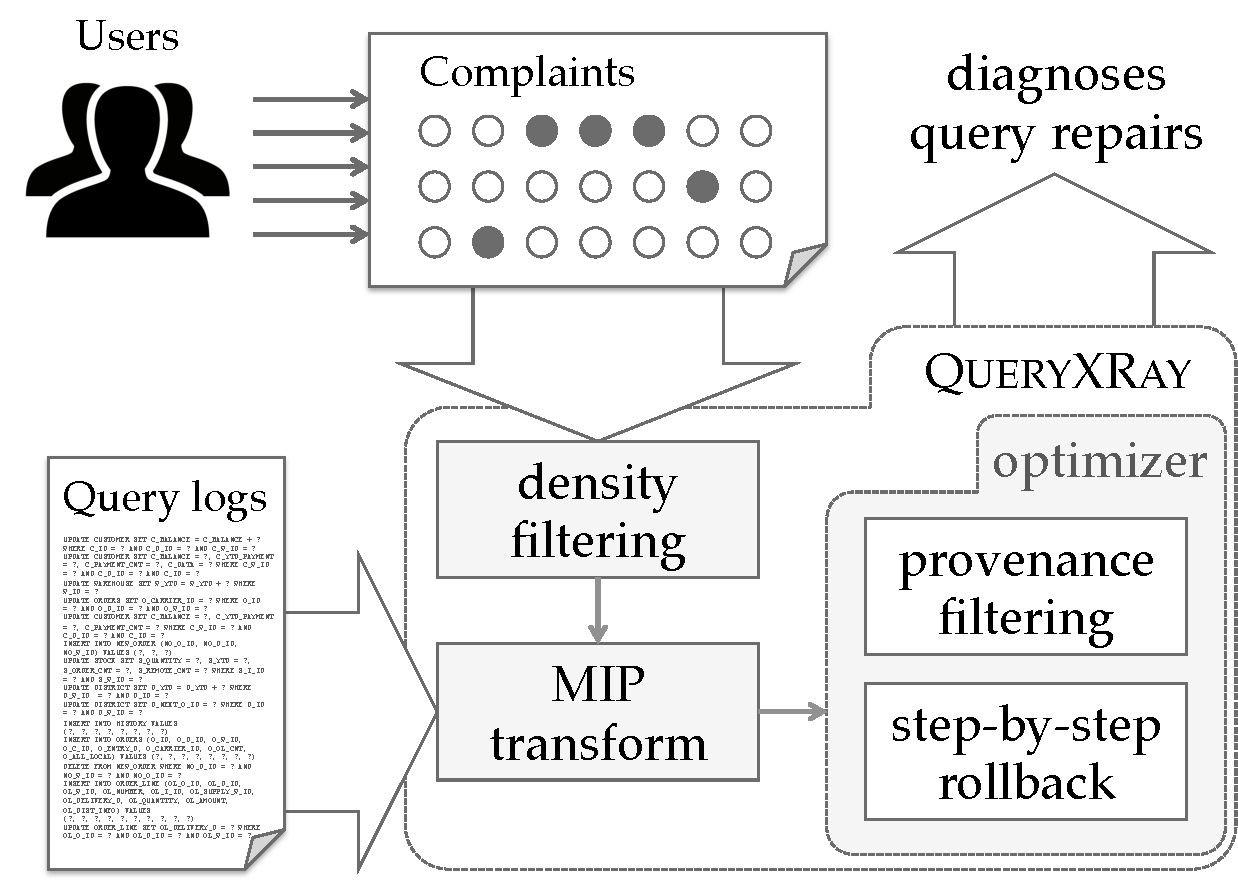
\includegraphics[scale=0.35]{figures/architecture}
    \caption{\sys processes data anomalies in the form of complaints and analyzes logged query histories to identify the causes of error. In the heart of the system, transformation algorithms express the diagnosis problem as a mixed integer program, and optimization modules ensure that the MIP programs can be evaluated efficiently.}
    \label{fig:architecture}
\end{figure}


\alex{Do we want to actually describe the architecture in a small section, or should we just include the figure in the front page?}


